%! Author = lsc
%! Date = 2021/1/9

%!TEX program = xelatex
% Preamble
\documentclass{cqupt_thesis}

% Packages
%\usepackage{showframe}


% Document
\begin{document}
%    ------论文信息填充
    \cntitle{重庆邮电大学硕士学位论文写作模板}
    \cnsubtitle{(写作模板)V1.1} % 论文题目太长,可以使用副标题
%    \cnsubsubtitle{长标题} % 论文题目还是太长,可以使用副副标题
    \entitle{Thesis Template for Master's}
    \ensubtitle{Degree of Chongqing University}
    \ensubsubtitle{of Posts and Telecommunications}
    \stuno{学号}
    \name{姓名}
    \degreeclass{工学硕士/理学硕士/工程硕士}
    \major{计算机技术}
    \supervisor{姓名\quad  职称}
    \completedate{2019年2月2日}
    \classifiedindex{TP391} % 分类号
    \udc{004} % udc
    \statesecrets{公开} % 密级
    \paperno{D-10617-308-(2020)-02048} % 学位论文编号



    \makecover % 制作封面
    \makestatement % 制作声明页

    \cnkeywords{学位论文,论文格式,规范化,模板} % 中文关键字
    \enkeywords{thesis, format, standardization, template} % 英文关键字

%    ------中文摘要内容
    \begin{cnabstract}

        学位论文是研究生从事科研工作的成果的主要表现,它集中表明了作者在研究工作中获得的新发明、新理论或新见解,是研究生申请学位的重要依据,也是科研领域中的重要文献资料和社会的宝贵财富。为了提高研究生学位论文的质量,做到学位论文在内容和格式上的规范化与统一化,特制作本模板。

        论文摘要是论文内容不加注释和评论的简短陈述,应以第三人称陈述,用语力求简洁、准确。中文摘要字数原则上为600-800字,外文翻译应与中文内容一致,一般不超过700个实词。摘要的编写应遵循下列原则:

        1. 摘要应具有独立性和自含性,即不阅读论文的全文,就能获得必要的信息。摘要是学位论文的浓缩,简明扼要地介绍了学位论文的主要内容、见解及结论。

        2. 摘要中要有数据、有结论,是一篇完整的短文,可以独立使用,可以引用。

        3. 摘要内容应尽可能包括原论文的主要信息,供读者确定有无必要阅读全文,也供文摘汇编等二次文献采用。

        4. 摘要一般应说明研究工作的目的意义、主要问题、研究内容、研究方法、研究结果、主要结论及意义、创造性成果和新见解,而重点是结果和结论。

        5. 摘要要用文字表达,不用图、表、化学结构式、公式、非公知公用的符号和术语、上下标以及其他特殊符号。

        关键词是为了文献标引工作从论文中选取出来用以表示全文主题内容信息的单词或术语。自定义3-5个关键词,按外延由大到小排列,建议采用EI标准检索词,关键词间用逗号分开。如有可能,应尽量用《汉语主题词表》等词表提供的规范词。

        “摘要”二字为黑体三号字居中,是一级标题。摘要与内容之间不空行,摘要内容与关键词间空一行。“关键词”三个字采用宋体小四号字加粗。摘要内容和关键词采用中文宋体、英文Times New Roman,小四号字,1.5倍行距。

    \end{cnabstract}


%    ------英文摘要内容
    \begin{enabstract}

        Thesis is postgraduate's main academic performance to display her/his works of scientific research, which shows the author's new invention, new theory or new opinion in her/his research. It is the crucial document for the graduate students to apply for degree, and it is also the important scientific research literature and the valuable wealth of society. In order to improve the quality of postgraduate's thesis, this template is formulated to standardize and unify the thesis's content and format.

        Abstract is a brief statement of the thesis without notes and comments, which should be stated in the third person with concise and accurate language in 600-800 Chinese characters and less than 700 words in foreign languages. The writing of an abstract should follow these principles:

        1. Abstract should be independent and self contained, which can offer the necessary information without reading the full text. It is the miniature and abbreviation of a thesis, which contains the thesis's main points, views and conclusions in a short and clear way.

        2. Abstract is a complete short essay with data and conclusion, which can be adopted and referred to independently.

        3. Abstract should include main information of the original thesis as far as possible for the reader to determine whether to read the full text, which can also be applied for secondary sources.

        4. Abstract should generally state out clearly the purpose, significance, problem, methods, results, main conclusion and its significance, creative achievements and new insights of the research program, and the results and conclusions should be emphasized.

        5. Abstract should be written in words without any appended drawings and photos. Unless there is no alternative way available, abstract should be presented without graphs, tables, chemical structural equations, non-public common symbols and terminology, subscripts, and other special symbols. It is the best policy to highlight the key points clearly with less data tables.

        Keywords are words or terms selected from the thesis for literature indexing to represent the topic information entry. Generally, a thesis should have 3-5 keywords, which should be arranged from broad to narrow entry according to the principle of epitaxial order. EI standard retrieval words are recommended. The keywords should be separated by a comma and there is no punctuation after the last word. If possible, it is better to use the standard words from \textit{Chinese Thesauri} and other dictionaries of the same type.

        Abstract should be centered in bold-3 word size. It is the primary heading without any blank line between the word “abstract” and its content. But there should be one blank line between the abstract content and the key words. The “keywords” should be in bold Song typeface with small-four word size. The content and the key words are written in Chinese song typeface, English Times New Roman, small-four word size and 1.5 spaced.

    \end{enabstract}

    % 制作目录,有点不优雅,后期优化。这样做能使dot line延伸至页码
%    https://tex.stackexchange.com/questions/134769/dotted-line-in-toc-despite-cftsetpnumwidth
    {\def\makebox[#1][#2]#3{#3}%
        \clearpage
        \makefancyhf{目录}
        \tableofcontents
        \thispagestyle{fancy}
    }
    {\def\makebox[#1][#2]#3{#3}%
        \clearpage
        \makefancyhf{图录}
        \listoffigures
        \thispagestyle{fancy}
    }
    {\def\makebox[#1][#2]#3{#3}%
        \clearpage
        \makefancyhf{表录}
        \listoftables
        \thispagestyle{fancy}
    }


%   ------注释表
    \makecommenttable{
        UDC & Universal Decimal Classification,国际十进分类法\\
        IMRAD & Introduction,Material and Method,Results,and Discussion(Conclusion)\\
        GPS & Global Positioning System,全球定位系统\\
        RFD & Reduced-function Device,精简功能设备\\
        RFID & Radio Frequency Identification,射频识别\\

    }


    \initmaincontent % 正文内容准备初始化


    \chapter{引言}

    制定本模板的目的是为了统一规范我校硕士学位论文的格式,保证学位论文的质量。本章说明了本模板的制定依据、学位论文要求、封面规范和以及学位论文中的引言目的、构成和写作要求。


    \section{格式模板的依据和使用说明}

    \subsection{学位论文模板依据}

    学位论文是研究生从事科研工作的成果的主要表现,它集中表明了作者在研究工作中获得的新的发明、理论或见解,是研究生申请学位的重要依据,也是科研领域中的重要文献资料和社会的宝贵财富。硕士学位论文应能表明作者已在本门学科上掌握了坚实的基础理论和系统的专业知识,并对所研究课题有新的见解,有从事科学研究工作或独立担负专门技术工作的能力[1] 。

    本模板主要参照《学位论文编写规则》(GB/T7713.1-2006,中国国家标准局2006年发布并实施)[1]、科学出版社出版的《作者编辑手册》[2]、全国科学道德和学风建设宣传教育领导小组制定的《科学道德与学风建设宣讲参考大纲(试用本)》(2011年11月)[3] 、《文后参考文献著录规则》(GB/T7714-2005,中国国家标准局2005年发布并实施)[4]等制定。

    部分范例来自《障碍环境中Swarm突现计算模型研究及行为控制》[5]等重庆邮电大学硕士学位论文。

    \subsection{本模板使用说明}
    本模板是2015年首次发布并将在重庆邮电大学研究生撰写硕士学位论文工作中推广。

    特别要说明的是,因为参考资料来源众多,首次发布的工作时间有限,引用内容可能存在标注不全、格式欠规范之处,敬请谅解。本文中凡有不规范或不明之处,以国家标准规范为准,研究生院负责解释。对发现的问题,将在后续版本中及时完善。

    本标准采用PDF、Word两种文本格式发布,满足大多数研究生和导师需要,便于师生交互式修订论文。其中,PDF版本为最终样式参考,如有不同,以此为准。为方便工作,广大研究生可直接采用Office 2013版,在本模板的Word文档中撰写论文,但应注意不要随意修改格式或刷新格式(因为Word软件的原因容易导致格式混乱),编辑从其他地方拷贝文字时应消除外来格式。下一步,除了对Word模板进行进一步的样式规范外,将陆续公布Latex、WPS等模板供研究生使用。


    \section{封面}

    \subsection{分类号、UDC编号、学位论文编号和密级}

    \subsubsection{分类号}
    分类号指中图分类号,是指采用《中国图书馆分类法》(原称《中国图书馆图书分类法》,简称《中图法》)对科技文献进行主题分析,并依照文献内容的学科属性和特征,分门别类地组织文献,所获取的分类代号。采用1999年出版的第四版《中图法》\footnote{
        中图分类号的类目名称:+ A马克思主义、列宁主义、毛泽东思想、邓小平理论;+ B哲学、宗教;+ C 社会科学总论;+ D政治、法律;+ E军事;+ F经济;+ G文化、科学、教育、体育;+ H语言、文字;+ I文学;+ J艺术;+ K历史、地理;+ N 自然科学总论;+ O 数理科学和化学;+ P天文学、地球科学;+ Q生物科学;+ R医药、卫生;+ S农业科学;+ T工业技术;TB一般工业技术;TD矿业工程;TE石油、天然气工业;TF冶金工业;TG金属学与金属工艺;TH机械、仪表工业;TJ武器工业;TK能源与动力工程;TL原子能技术;TM电工技术;TN无线电电子学、电信技术;TP自动化技术、计算机技术;TQ化学工业;TS轻工业、手工业;TU建筑科学;TV水利工程;+ U交通运输;+ V航空、航天;+ X环境科学、安全科学;+ Z 综合性图书。}可以在http://www.33tt.com/tools/ztf(中国图书馆分类法中图分类号查询系统)或http://lib.jzit.edu.cn/sjk/tsflf/index.htm(中图法第四版计算机辅助分类查询系统)中查询。填写要求:要求分类细分到22个大类代码后三位数字。如:TN929。

    \subsubsection{UDC编号}
    UDC即国际十进分类法(Universal Decimal Classification),是国际通用的多文种综合性文献分类法。UDC采用单纯阿拉伯数字作为标记符号。它用个位数(0~9)标记一级类,十位数(00~99)标记二级类,百位数(000~999)标记三级类,以下每扩展(细分)一级,就加一位数。每三位数字后加一小数点。如电气工程类的论文,其UDC编号为:621.3。


    \chapter{正文内容及文字格式}
    论文正文是主体,是学位论文的核心部分,占主要篇幅。本章说明论文正文的组成部分、写作要求和方法以及论文的字数要求。


    \section{论文正文}
    论文内容一般应由10个主要部分组成,依次为:封面,中文摘要,英文摘要,目录,图录、表录、注释表,论文正文,参考文献,附录,致谢,攻读学位期间发表的成果目录。

    论文正文占主要篇幅。一般由标题、文字叙述、图、表格和公式等5个部分构成。写作形式可因研究课题性质不同而变化,论文正文一般包括:引言(或绪论)、文献综述(可在引言部分给出)、理论基础、计算方法、实验装置和测试方法,经过整理加工的实验结果的分析讨论、见解和推论,与理论计算结果的比较以及本研究方法与已有研究方法的比较等。要求概念清晰,数据可靠,分析严谨,立论正确,要能反映出学位论文的学术水平。


    \section{字数要求}
    硕士学位论文字数一般不少于3万字。但论文撰写不严格限制必须3万字以上,以实际撰写内容是否完备、体现水平为参考依据。一般情况下,论文全部篇幅不少于40页,其中以论文工作描述为主(正文章节内容至少占全部篇幅75%)。


    \chapter{注释、图表、公式和计量单位格式}


    \section{图表格式}
    表注主要包括三种情况:资料来源(说明表中数据的文献来源,可用标题上引用参考文献、表下说明出处或脚注三种方式之一给出)、普通注解(对表中的数据处理的说明)、特殊注解(对某一个或几个表栏项目进行特别说明),如表\ref{电流类型对效率的影响}所示。
    \begin{table}[H]% H代表就插在此位置
        \centering
        \caption{电流类型对效率的影响}
        \label{电流类型对效率的影响}
        \begin{tabular}{p{3.5cm}p{3.5cm}p{3.5cm}p{3.5cm}}
            \hline
            电流类型           & {$ A_1^* $} & {$ W_{bc}/W_k^{**} $} & {g/\%}   \\
            \hline
            {$ J^2(t)=1 $} & 4.27        & 1.28                  & 43.9(30)            \\
            {$ J^2t=1 $}   & 4.64        & 1.39                  & 41.8(29)            \\
            {$ J^2t=1-t $} & 3.28        & 0.98                  & 50.5     \\
            \hline
            \multicolumn{4}{p{15cm}}{
                资料来源:Wang Ying et al.2004.Physics of Electric Launch.Science Press。

                注:括号内的数字表明了$ W_{in}\neq0 $的情况;*表示$ v_{p0}/v_{pf}=0 $,**表示$ h=20mm,L_rL_r^\prime=0.628\mu H/m,l_g=2m,v_{pf}=3km/s $。
            }
        \end{tabular}
    \end{table}
    表名中不允许使用标点符号,表名后不加标点。表名与正文之间不空行。数字空缺的格内加横线“-”(占2个数字宽度)。

    表内文字或数字上、下或左、右相同时,采用通栏处理方式(合并单元格),表内文字或数字上、下或左、右相同时,采用通栏处理方式(合并单元格),或一律填上具体数字或文字,不允许用“〃”“同上”之类的写法。


    \begin{figure}[H]
        \centering

        \subfigure[\zihao{5}平均个体聚类度变化图]{
            \begin{minipage}[t]{0.5\linewidth}
                \centering
                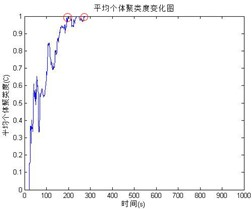
\includegraphics[width=5cm]{figs/图片1}
                %\caption{fig1}
            \end{minipage}%
        }%
        \subfigure[\zihao{5}邻域个体分布指数变化图]{
            \begin{minipage}[t]{0.5\linewidth}
                \centering
                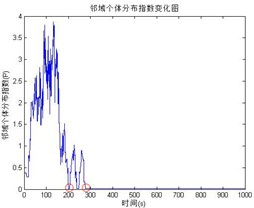
\includegraphics[width=5cm]{figs/图片4}
                %\caption{fig2}
            \end{minipage}%
        }%

        \centering
        % 这样做图录里可以避免出现文献上标
        \caption[标示群体突现时刻的指标变化图]{ 标示群体突现时刻的指标变化图\cite{陈浩元2015gb} }
    \end{figure}
    曲线图的纵横坐标必须标注“量、标准规定符号、单位”。此三者只有在不必要标明(如无量纲等)的情况下方可省略。坐标上标注的量的符号和缩略词必须与正文一致。


    \chapter{其他格式}


    \section{数学环境}
    \begin{theorem}[Lindeberg--Lévy 中心极限定理]
        设随机变量 $X_1, X_2, \dots, X_n$ 独立同分布, 且具有期望 $\mu$ 和有限的方差 $\sigma^2 \ne 0$,
        记 $\bar{X}_n = \frac{1}{n} \sum_{i+1}^n X_i$,则
        \begin{equation}
            \lim_{n \to \infty} P \left(\frac{\sqrt{n} \left( \bar{X}_n - \mu \right)}{\sigma} \le z \right) = \Phi(z),
        \end{equation}
        其中 $\Phi(z)$ 是标准正态分布的分布函数。
    \end{theorem}
    \begin{proof}
        Trivial.
    \end{proof}


    \section{插入代码}
    % 代码环境
    其他数学环境定义对应命令:
    \begin{lstlisting}[language = java, numbers=left,
    numberstyle=\tiny,keywordstyle=\color{blue!70},
    commentstyle=\color{red!50!green!50!blue!50},frame=shadowbox,
    rulesepcolor=\color{red!20!green!20!blue!20},basicstyle=\ttfamily]

	\newtheorem{assumption}{假设}[chapter]
    \newtheorem{definition}{定义}[chapter]
    \newtheorem{proposition}{命题}[chapter]
    \newtheorem{lemma}{引理}[chapter]
    \newtheorem{theorem}{定理}[chapter]
    \newtheorem{axiom}{公理}[chapter]
    \newtheorem{corollary}{推论}[chapter]
    \newtheorem{exercise}{练习}[chapter]
    \newtheorem{example}{例}[chapter]
    \newtheorem{remark}{注释}[chapter]
    \newtheorem{problem}{问题}[chapter]
    \newtheorem{conjecture}{猜想}[chapter]

    \end{lstlisting}


    \section{算法}

    \begin{algorithm}[H]

        \label{用归并排序求逆序数}
        \caption{用归并排序求逆序数}
        \begin{algorithmic}[1] %每行显示行号
            \Require $Array$数组,$n$数组大小
            \Ensure 逆序数
            \Function {MergerSort}{$Array, left, right$}
                \State $result \gets 0$
                \If {$left < right$}
                    \State $middle \gets (left + right) / 2$
                    \State $result \gets result +$ \Call{MergerSort}{$Array, left, middle$}
                    \State $result \gets result +$ \Call{MergerSort}{$Array, middle, right$}
                    \State $result \gets result +$ \Call{Merger}{$Array,left,middle,right$}
                \EndIf
                \State \Return{$result$}
            \EndFunction
            \State
            \Function{Merger}{$Array, left, middle, right$}
                \State $i\gets left$
                \State $j\gets middle$
                \State $k\gets 0$
                \State $result \gets 0$
                \While{$i<middle$ \textbf{and} $j<right$}
                    \If{$Array[i]<Array[j]$}
                        \State $B[k++]\gets Array[i++]$
                    \Else
                        \State $B[k++] \gets Array[j++]$
                        \State $result \gets result + (middle - i)$
                    \EndIf
                \EndWhile
                \While{$i<middle$}
                    \State $B[k++] \gets Array[i++]$
                \EndWhile
                \While{$j<right$}
                    \State $B[k++] \gets Array[j++]$
                \EndWhile
                \For{$i = 0 \to k-1$}
                    \State $Array[left + i] \gets B[i]$
                \EndFor
                \State \Return{$result$}
            \EndFunction
        \end{algorithmic}
    \end{algorithm}



    \begin{reference}
        \bibliography{ref}
    \end{reference}


    \beginappendix


    \chapter{科技写作中非学术性低级错误的主要表现}

    本附录主要针对学位论文写作或中文科技论文写作,供重庆邮电大学硕士学位论文查非工作参考。未尽事宜,可参考重庆邮电大学论文写作要求、重庆邮电大学学报编辑部等国内期刊社、出版社的通用出版规定。

    推荐阅读《科学出版社作者编辑手册》、《科学道德与学风建设宣传参考大纲(试用本)》等写作指导性书籍或资料,可了解更多、更详尽的通用写作出版规范。


    \chapter{中国科协关于科技工作者科学道德规范(试行)}


    \section{总 则}
    第一条 为弘扬科学精神,加强科学道德和学风建设,提高科技工作者创新能力,促进科学技术的繁荣发展,中国科学技术协会根据国家有关法律法规制定《科技工作者科学道德规范》。

    第二条 本规范适用于中国科学技术协会所属全国学会、协会、研究会会员及其他科技工作者。

    第三条 科技工作者应坚持科学真理、尊重科学规律、崇尚严谨求实的学风,勇于探索创新,恪守职业道德,维护科学诚信。

    第四条 科技工作者应以发展科学技术事业,繁荣学术思想,推动经济社会进步,促进优秀科技人才成长,普及科学技术知识为使命,以国家富强,民族振兴,服务人民,构建和谐社会为己任。


    \section{学术道德规范}

    第五条 进行学术研究应检索相关文献或了解相关研究成果,在发表论文或以其他形式报告科研成果中引用他人论点时必须尊重知识产权,如实标出。

    第六条 尊重研究对象(包括人类和非人类研究对象)。在涉及人体的研究中,必须保护受试人合法权益和个人隐私并保障知情同意权。

    第七条 在课题申报、项目设计、数据资料的采集与分析、公布科研成果、确认科研工作参与人员的贡献等方面,遵守诚实客观原则。对已发表研究成果中出现的错误和失误,应以适当的方式予以公开和承认。

    \begin{acknowledgements}
        致谢二字一级标题:黑体3号字居中,段前17磅,段后16.5磅,1.5倍行距,致谢二字与致谢内容之间不空行。致谢内容正文样式:宋体小四号,1.5倍行距。

        可以从下列方面致谢:
        对国家科学基金、资助研究工作的奖学金基金、合同单位、资助或支持的企业、组织或个人;

        对协助完成研究工作和提供便利条件的组织或个人;

        对在研究工作中提出建议和提供帮助的人;

        对给予转载和引用权的资料、图片、文献、研究思想和设想的所有者;

        对其他应感谢的组织或个人。主要感谢导师和对论文工作有直接贡献及帮助的人士和单位。学位申请人的家属及亲朋好友等与论文无直接关系的人员,一般不列入致谢的范围。

        致谢辞应谦虚诚恳,实事求是,切忌浮夸与庸俗之词。

    \end{acknowledgements}

    \begin{mastermainwork}
        \section*{参与科研项目:}
        \begin{achievements}
            \item 项目名称(编号),项目类别,项目起止
        \end{achievements}

        \section*{发表及完成论文:}
        \begin{achievements}
            \item 个人成果包括论文、专利等,和毕业条件、信息系统里一致。同参考文献要求。完成人姓名用加粗。样例如下条。
            \item \textbf{郝某}, 井某, 张某. 论文题目[J]. 期刊名称, 2014, 29(11): 1521-1524.
        \end{achievements}
    \end{mastermainwork}


\end{document}